% !TEX root = ../main.tex
% chktex-file 21
% chktex-file 46
\section{Spectral Graph Theory}%
\label{sec:sgt}

We start with an introduction to spectral graph theory, which will allow us to characterize and compare the structure of graphs.
Graphs are most commonly described in their vertex base, i.~e.\@ the strength $w_{i j}$ with which pairs $(v_i, v_j)$ of vertices are connected.
\begin{align*}
	G :=&\, (\mathcal{V}, \mathcal{E}, W) \text{ with } W \in \mathbb{R}^{N \times N}, N := |\mathcal{V}|
\end{align*}
In this paper we will only consider undirected graphs with non-negative real weights; thus the adjacency matrix $W$ is positive semi-definite.

The core idea of spectral graph theory is to perform a change of basis of $W$ and describe graphs in terms of their so called \textit{spectral base} instead of their \textit{vertex base}.
To see what this means, we interpret the adjacency matrix $W$ as a linear operator that operates on so called signals $x \in \mathbb{R}^N$.
A signal $x$ can be interpreted as a function $x: \mathcal{V} \to \mathbb{R}$ that assigns a signal strength to each vertex.
By applying $Wx$ the given signal strengths $x_i$ are shifted according to the connection strenghts $w_{i j}$ to neighboring vertices $v_j$.
This interpretation of graphs is very similar to that of Markov chains where signals represent probability distributions.

\subsection{Relating Graph Signals to Real Functions}%
\label{sec:sgt:real}

Let us now compare discrete graph signals $x: \mathcal{V} \to \mathbb{R}$ to continuous real functions $f: \mathbb{R} \to \mathbb{R}$.
Both only differ in their domain.
The domain $\mathbb{R}$ of $f$ has an inherent structure, the real number line, which provides a strict ordering of its elements and a notion of distance between them.
The domain $\mathcal{V}$ of $x$ however has no such inherent structure, i.~e.\@ $v_1 < v_2$ for two vertices $v_1, v_2$ does not have a clear meaning.
The structure of $\mathcal{V}$ fully depends on the graph $G$ that is acting on it.
Intuitively graph signals can thus be understood as a discretized generalization of real functions, where the underlying structure of the input domain is not fixed but can be freely chosen.
\begin{figure}
	\centering
	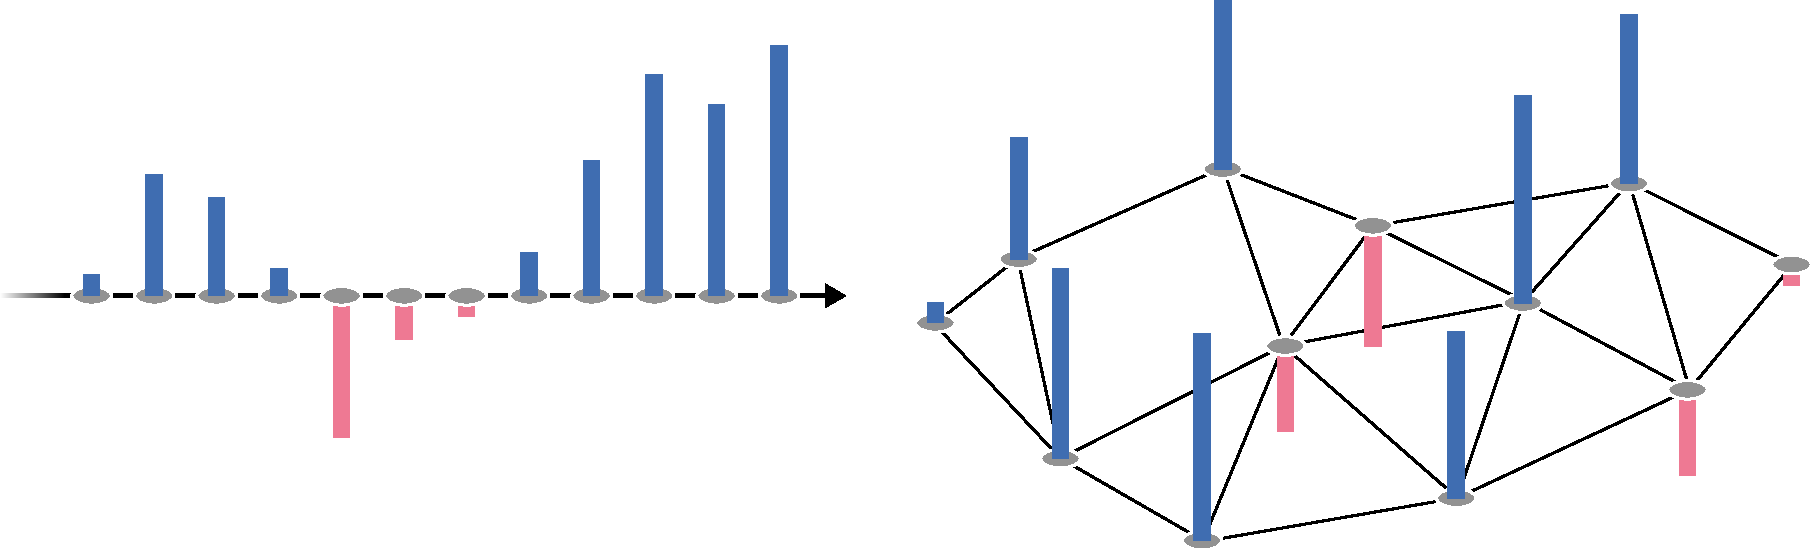
\includegraphics[width=0.9\linewidth]{gfx/sgt/real-graph.pdf}
	\caption{
		Illustration of how the discretized real number line can be interpreted as an infinite linear graph, compared to some arbitrary finite non-linear graph.
		The bars show the signal strengths $f(t)$ and $x_i$ at the vertices $b_t$ and $b_i$ respectively.
	}\label{fig:sgt:realGraph}
\end{figure}
Figure~\ref{fig:sgt:realGraph} shows that all real functions $f$ can be seen as signals $x$ of the graph described by the real number line\footnote{
	Technically this is not correct, since $\mathbb{R}$ is continuous whereas all vertex sets $\mathcal{V}$ have to be discrete.
	To build an intuition for graph signals, this detail can however be ignored.
}.
Both, real functions and graph signals, can be described as vectors in their vertex base:
\begin{equation}
	\begin{split}
		f = \int_{\mathbb{R}} f(t) b_t dt
		\Rightarrow \langle b_t, f \rangle = f(t)
	\end{split}
	\quad\text{and}\quad
	\begin{split}
		x = \sum_{i = 1}^{N} x_i b_i
		\Rightarrow \langle b_i, x \rangle = x_i
	\end{split}
\end{equation}
In this equation ${\{ b_i \}}_{v_i \in \mathcal{V}}$ denotes the standard basis of the adjacency matrix $W$.
Similarly ${\{ b_t \}}_{t \in \mathbb{R}}$ denotes the infinite dimensional standard basis of the space of real functions, where $\langle b_t, \cdot \rangle := \delta_t(\cdot)$, with $\delta$ denoting the Dirac delta function.

\subsection{Extending the Fourier Transform to Graphs}%
\label{sec:sgt:fourier}

As mentioned at the beginning of this section, the core idea of spectral graph theory is to express graph signal vectors $x$ in the spectral basis ${\{ u_i \}}_{i = 1}^{N}$ instead of the standard vertex basis ${\{ b_i \}}_{v_i \in \mathcal{V}}$.
This idea is analogous to the classical Fourier transform on real-valued functions.
In the first step we are now going to give an intuition for the classical Fourier transform.
Afterwards we will extend this intuition to the graph domain.

The Fourier basis ${\{ u_\xi \}}_{\xi \in \mathbb{R}}$ describes a function $f$ not in terms of the values $f(t) = \langle b_t, f \rangle$ it takes at position $t$ but instead in terms of the amplitudes $\hat{f}(\xi) = \langle u_\xi, f \rangle$ of the complex exponentials $u_\xi(t) = e^{2\pi i \xi t}$.
Using this perspective, the Fourier transform can be viewed as a change of basis operator from the orthonormal standard basis ${\{ b_t \}}_{t \in \mathbb{R}}$ to the also orthonormal Fourier basis ${\{ u_\xi \}}_{\xi \in \mathbb{R}}$:
\begin{align}
	f = \int_{\mathbb{R}} \underbrace{\langle b_t, f \rangle}_{f(t)} b_t dt = \int_{\mathbb{R}} \underbrace{\langle u_\xi, f \rangle}_{\hat{f}(\xi)} u_\xi d\xi
\end{align}
This property of the Fourier transform by itself is not special; in fact there are infinitely many orthonormal bases on the space of real-valued functions.
The distinguishing property of ${\{ u_\xi \}}_{\xi \in \mathbb{R}}$, making it useful in many domains, is that it is an \textit{eigenbasis} of the \textit{Laplacian} $\ma\Updelta$, i.~e.\@ $\Updelta u_\xi = \lambda_\xi u_\xi$ for $\lambda_\xi \in \mathbb{R}$.
The Laplacian is a multi\-dimensional generalization of the second derivative.
For real-valued functions this boils down to $\Updelta u_\xi = \frac{\partial^2}{\partial t^2} u_\xi = -{(2 \pi \xi)}^2 e^{2 \pi i \xi t}$.
The original motivation to express functions in terms of the Laplacian's eigenbasis was to solve the physical heat equation\footnote{
	More generally the Fourier basis turns out to be meaningful for all \textit{linear time-invariant} (LTI) systems, of which the heat equation is only one instance.
}.
For this reason it is a useful intuition to think about signals as temperature distributions that will converge to an equilibrium state over time.
This intuition also works in the graph setting where heat only flows between neighboring vertices in proportion to their connection strengths.

Now, that we have looked at the Fourier transform of real-valued functions, we will extend this notion to graphs.
Just like the classical Fourier transform, the graph Fourier transform performs a change of basis of a signal $x$ from the vertex basis ${\{ b_i \}}_{v_i \in \mathcal{V}}$ to the Fourier basis ${\{ u_k \}}_{1 \leq k \leq |\mathcal{V}|}$.
This Fourier basis again is characterized by it being an eigenbasis of the Laplacian, more specifically the so called \textit{combinatorial graph Laplacian} $L$ in this case.
\begin{align}
	L := D - W \text{ with } D :=
\end{align}

\begin{figure}
	\centering
	\makebox[\textwidth][c]{\includegraphics[width=\linewidth]{gfx/sgt/graph-fourier.pdf}}
	\caption{
		x
	}\label{fig:sgt:graphFourier}
\end{figure}
